\documentclass{article}
\usepackage[left=2.5cm, right=2.5cm, top=3cm, bottom=3cm]{geometry}
 \usepackage{graphicx}
\renewcommand{\abstractname}{}
\begin{document}
\title{ \textbf{HULK} (Proyecto de Pogramación II)}
\author{ Laura Alonso Rivero C-113}
\date{}
\maketitle
\rule{1.0\textwidth}{0.1mm}

\begin{flushleft}
\begin{abstract}
\begin{center}
\textbf{¿Qué es HULK ?}
\end{center}
\textbf{`HULK`}, o Havana University Languaje by Kompilers, por sus siglas en inglés es un lenguaje de programación imperativo, funcional, estática y fuertemente tipado. En este proyecto se ha implementado un subconjunto de \textbf{ HULK} el cual se compone solamente de expresiones que pueden escribirse en una línea.
El intérprete de \textbf{ HULK} será una aplicación de consola, donde el usuario puede introducir una expresión presionar  \textbf{ ENTER}, e inmediatamente se verá el resultado de evaluar la expresión en caso de que lo hubiera. El proceso se continuará ocurriendo hasta que el usuario presione \textbf{Ctrl + C}.
\end{abstract}

\large {Al iniciar la aplicación el usuario tiene dos opciones:}
\begin{itemize}
\item \large {En caso de no conocer el funcionamiento de la aplicación puede presionar ' h ' y se imprimirá en la consola todas las posibles expresiones que puede declarar con este lenguaje.}
\item \large {Si conoce el funcionamiento y si  desea comenzar puede presionar ' s '  de este modo se inicia el proceso de compilación.}
\end{itemize}
\end{flushleft}

\begin{figure}
[!h]\label{Opciones}
\centering
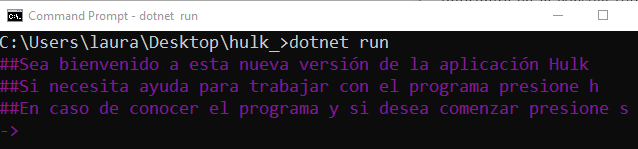
\includegraphics[width = 0.8\textwidth]{Opciones.png}
\caption{Opciones}
\end{figure}

\begin{flushleft}
\large{El proyecto consta de tres pasos fundamentales en su proceso de compilación:}
\begin{itemize}
 \item \large{Lectura de la expresión introducida por el usuario. De este proceso se encarga el  \textbf{ Lexer} el cual escanea la entrada y devuelve una lista de \textbf{Tokens}.}
\item \large{Creación del Árbol de Sintaxis Abstracta, AST por sus siglas en inglés. Esta parte corre por el \textbf{Parser} que devuelve una lista donde se clasifican las diferentes expresiones.}
\item \large{La interpretación de la expresión. Llevada a cabo por el  \textbf{Interpreter} que va a devolver la evaluación de la expresión entrada por el usuario.}
\end{itemize}

\Large {\textbf{Lectura de la expresión (Ánalisis Léxico)}}\linebreak \\
\large {Cuando el usuario introduce la línea comienza la lectura de la expresión, con este propósito se creó la clase \textbf{ Lexer}. Esta clase consta de un método principal llamado \textbf{Scan} el cual recorre cada  caracter de la entrada del usuario y dependiendo de sus valores se irán clasificando. Esta clasificación está dada debido al tipo de \textbf{Token} que sea.}\linebreak \\
\large {Un  \textbf{Token} es una secuencia de caracteres que posee un valor y tipo específico. Existen diversos tipos como son: las palabras claves (print, let, if), los nombres de las variables o las funciones (x, y, fib), los operadores aritméticos, de relación y lógicos (*, ==, \&), las funciones matemáticas (cos, sqrt, log) y finalmente los literales numéricos, cadenas de strings o booleanos. Estos están agrupados en un enum nombrado \textbf{TypesOfToken}. Para guardar todos los tokens específicos del lenguaje se creó un diccionario \textbf{Tokens} que posee como valor el tipo de \textbf{Token} que es y su valor y cuya llave es un string que será el valor del  \textbf{Token}.}\linebreak \\
\large {Una vez escaneada toda la entrada se devolverá una lista con todos estos tokens en la posición en que fueron encontrados para su posterior procesamiento.}\linebreak \\

\Large {\textbf{Creación del AST  (Ánalisis Sintáctico)}}\linebreak \\
\large {A partir de la lista de Tokens retornada se procede a crear el Árbol Sintáctico el cual no es más que una forma de definir los pasos a seguir por el Compilador a la hora de evaluar las expresiones de una forma recursiva. En este caso se uso el método de parsing recursivo descendente, el cual  consiste en construir el árbol a partir de las reglas de gramática de cada lenguaje.  Esta grámatica se encuentra implementada en la clase \textbf{Parser} y sigue la siguiente estructura:}\linebreak \\
\end{flushleft}

\begin{figure}
[!h]\label{Gramática}
\centering
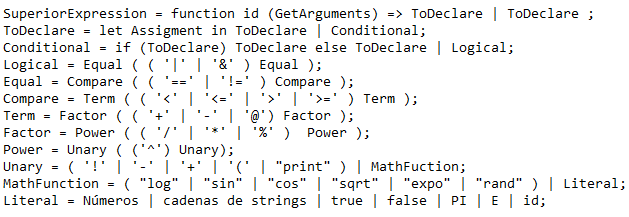
\includegraphics[width =0.9\textwidth]{Gramática.png}
\caption{Gramática}
\end{figure}

\begin{flushleft}
\large {Con este método de parsing se comienza a partir del símbolo inicial (raíz) y se va descendiendo en el AST hacia las hojas. En cada caso se elige la regla gramatical adecuada y se invoca la función correspondiente para continuar el análisis.}\linebreak \\
\large {Para lograr la generación del árbol fue necesario crear la clase abstracta \textbf{Expression} para poder identificar los distintos tipos de expresiones que el usuario era capaz de implementar y agregarlas a una lista. Al ser abstracta toda aquella clase que la herede podrá contar con los métodos que posee. En este caso el único método a heredar es utilizado en la evaluación de las expresiones.}\linebreak \\

\Large {\textbf{Interpretación de la expresión  (Ánalisis Semántico)}}\linebreak \\
\large {En esta etapa se interpreta, evalúa y finalmente se devuelve el resultado de la entrada del usuario a través de la clase \textbf{Interpreter}. El objetivo es verificar que las operaciones sean realizadas con los operandos correctos.}\linebreak \\
\large {En algunas expresiones como la declaración de variables y funciones fue necesaria la creación de un \textbf{Scope global}. Esto no es más que el conjunto de variables o funciones que son accesibles desde cualquier parte del programa. Es muy importante para evitar conflictos y ambigüedades en el código pues una vez declarada una función o variable no es posible declarar una con el mismo nombre en el mismo ámbito y con las mismas características}\linebreak \\
\large {Para interpretar las expresiones se invoca el método \textbf{Evaluate} el cual como su nombre indica realiza la evaluación de los distintos tipos de expresiones guardados en la lista. Para ello se implementó la interfaz \textbf{Helper} que genera distintos métodos para evaluar cada expresión según sus particularidades.}\linebreak \\
\large {Una vez evaluada la entrada el resultado se imprimirá en la consola.}\linebreak \\

\Large {\textbf{Errores}}\linebreak \\
\large {En el lenguaje HULK existen tres tipos distintos de errores que se producen en cada etapa del proceso:}\linebreak \\
\large {Error Léxico: se presenta cuando las expresiones contienen caracteres no válidos en el lenguaje.}\linebreak \\
\large {Error Sintáctico: se presenta cuando la secuencia de tokens no es válida atendiendo a la gramática del lenguaje o cuando se trata de sobreescribir una variable o función en un mismo contexto.}\linebreak \\
\large {Error Semántico: se presenta cuando no se puede evaluar la expresión debido a incoherencias entr la operación y  los tipos de expresiones que se encuentra en ella.}\linebreak \\

\large {Con el correcto funcionamiento de esta aplicación considerada un compilador de una versión más simple del lenguaje \textbf{HULK}, se puede afirmar la capacidad para leer, interpretar y evaluar operaciones con instrucciones que posean cualquier tipo de las estructuras permitidas (operación aritmética,  llamado de funciones, declaración de funciones, condicionales, e incluso evaluar funciones con implementación recursiva).}\linebreak \\
\end{flushleft}

\end{document}